\documentclass{article}
\usepackage{graphicx}
\graphicspath{ {./images/} }
\usepackage[utf8]{inputenc}

\title{Rapport Technique Projet IAT}
\author{Agnès Thouvenin, Louis Gombert, Antoine Merle}
\date{30 Avril 2022}

\begin{document}

\maketitle

\section{Introduction et Objectifs}
Ce projet d'IAT consiste en la résolution autonome d'un problème en Intelligence Artificielle en utilisant l'apprentissage par renforcement. Dans notre cas, le problème à résoudre est le jeu de Space Invaders. 
\newline

Le but de ce jeu est que l'agent (un vaisseau) survive en tuant le plus d'aliens envahisseurs possibles. L'agent peut effectuer 4 actions différentes qui sont : aller à gauche, aller à droite, tirer ou ne rien faire. Par ailleurs, un alien tué rapporte une récompense et le but de l'agent est donc de maximiser la somme des récompenses perçues.
\newline

Initialement, les actions de cet agent sont sélectionnées totalement aléatoirement. L'objectif du projet est donc d'utiliser un algorithme d'apprentissage pour que l'agent réalise les meilleurs actions et obtienne ainsi le meilleur score.
\newline

Pour cela, nous avons commencé par définir les paramètres pour décrire l'état du problème. Dans un deuxième temps, nous avons mis en place l'algorithme d'apprentissage choisi. Finalement, nous avons monitoré l'apprentissage de l'agent afin de pouvoir optimiser l'apprentissage.

\section{Description de l'état}
La première étape dans cette résolution autonome est d'établir les paramètres pour définir l'état de ce problème d'apprentissage. Plus le nombre et la dimension des paramètres seront grands et plus la définition du problème sera précise. Cependant les états possibles seront très nombreux ce qui ralentira beaucoup l'apprentissage, car notre matrice Q sera trop grande. 
\newline

Il est donc important de trouver un juste milieu entre précision dans la définition du problème et la vitesse d'apprentissage. Nous avons donc choisi de définir l'état du processus d'apprentissage selon les paramètres suivants :
\begin{itemize}
\item le delta entre la position en X de l'agent et celle des ennemis (en Y). Ce delta est quantifié linéairement, avec un pas qui est un paramètre testé dans une partie ultérieure. Avec un pas trop important, on constate des effets de bloc, avec un vaisseau qui se déplace visuellement entre les bornes. Avec un pas trop faible, l'espace est trop important et l'apprentissage est plus long sans être forcément de meilleure qualité.
\item position en Y du monstre le plus bas quantifié non linéairement avec les bornes [-20, 150, 250] (3 espaces possibles, donc 3 dimensions). La grille utilisée ici est moins précise, ce qui n'est pas un problème car la position Y de l'ennemi va seulement influencer le timing du tir de l'agent.
\item déplacement de l'agent à gauche ou à droite de l'ennemi (booléen, 2 dimensions)
\item possibilité pour l'agent de tirer ou non (booléen, 2 dimensions)
\end{itemize}

Le nombre d'états est ainsi de $(G \cdot 3)^{N} \cdot 2 \cdot 2$, pour G le nombre de sections en $X$ et $N$ le nombre d'ennemis en jeu. Cet espace d'états sera assez restreint, mais nous verrons qu'il est suffisant pour parvenir à des résultats convaincants.


\section{Choix de l'algorithme}

L'algorithme que nous avons choisi de mettre en place pour résoudre ce problème d'apprentissage est l'algorithme de Q-learning.
\newline
D'après le cours, nous avons vu l'algorithme suivant :
\newline

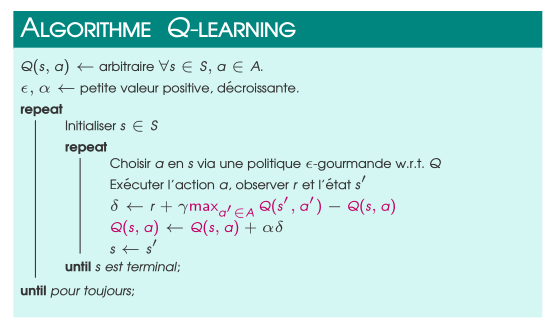
\includegraphics[scale=0.5]{pote.png}

\newline
avec \textbf{Q(s,a)} = définie la mesure de performance d'une paire état-action

\textbf{$\epsilon$} = taux d'exploration des possibilités (la part d'aléatoire dans le choix du modèle

\textbf{$\alpha$} = pas d'apprentissage de l'algorithme de la descente de gradient ; (sa valeur est fixée à 0.01) 

\textbf{s'} = l'état au pas suivant
\newline

Cet algorithme se base sur l'algorithme de la descente de gradient pour déterminer sa politique optimale.

\section{Monitoring de l'apprentissage}

Passons à l'optimisation des hyper-paramètres pour un apprentissage optimal. En plus d'epsilon, gamma et alpha, nous jouons avec le nombre d'épisodes utilisés pour l'apprentissage, le nombre de pas par épisode, et la granularité de l'état décrivant le delta en X. Nous lançons pour chaque set de paramètre testés 4 simulations, dont nous utilisons la moyenne du score pour déterminer son efficacité.

Nous avons essayé automatiquement grâce à un script python plusieurs sets de paramètres en les faisant varier un par un, pour tenter de trouver une combinaison acceptable. Empiriquement, la moyenne du score est la meilleure (sans problématique de temps de calcul) pour 5000 épisodes de 500 steps, avec un gamma de 0.99, un alpha (pas d'apprentissage de 0.01 et un epsilon de (taux d'exploration) de 0.01. Le détail des exécutions est à retrouver joint à ce rapport. Toutes les simulations ont été faites avec un seul ennemi.

\section{Évolution de la fonction de valeur Q}

Nous traçons un graphique de l'évolution du changement de Q au cours de l'apprentissage, par épisode : \newline

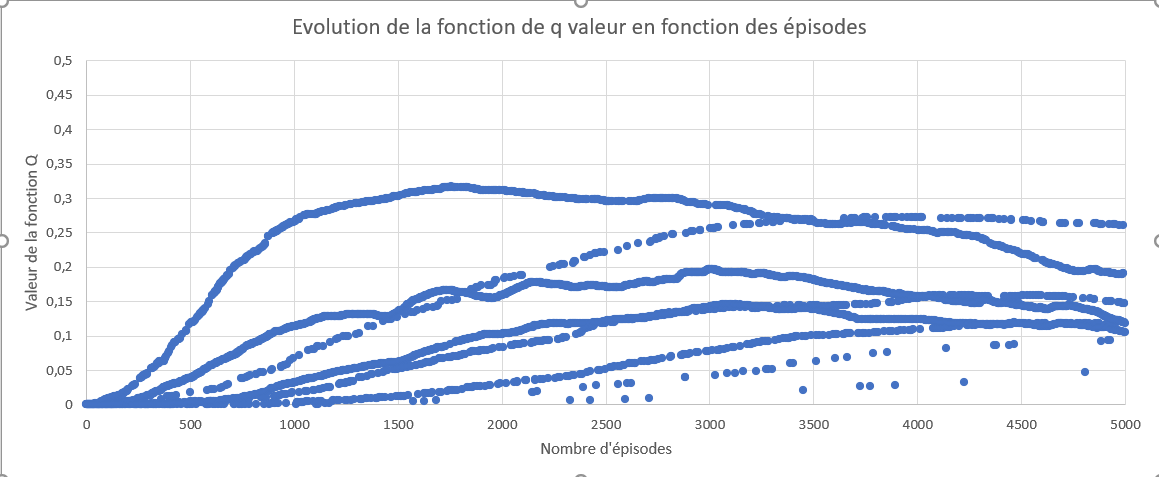
\includegraphics[scale=0.35]{graphe.png}


\newline

Les données utilisées pour réaliser ce graphique sont également joint au rapport dans le fichier logQ.csv.
\end{document}
